\documentclass[a4paper]{article}

\usepackage{graphicx}
\usepackage{amsmath}
\usepackage{natbib}
\usepackage{amsmath}
\usepackage[english]{babel}
\usepackage{graphicx}
\usepackage{amssymb}
\usepackage{graphicx}
\usepackage{url}
\usepackage{listings}
\usepackage{paralist}
\usepackage{color}
\usepackage{epstopdf}

\date{}

\begin{document}

\section{Application}
The use of the proposed methodology is demonstrated on data from the aforementioned HPV-induced transformation study. Primary interest is unravelling temporal and contemporaneous relations among the genes. Analysis and results, alongside with several down-stream explorations, are discussed and presented.

The data stem from an $\textit{in  vitro}$ HPV-immortalized cell line experiment. The employed cell line model faithfully mimics cervical cancer development, morphologically and (epi)genetically (\cite{Steenbergen2004}; \cite{Wilting2006}; \cite{Henken2007}). The experiment comprise four cell lines, two with HPV16 and two with HPV18 (\cite{Steenbergen1996}). Over time the cell lines undergo transcriptomic changes. Using oligonucleotide microarrays cell lines are assayed at eight sequential time points in order to assess these changes in mRNA levels. The preprocessing of the resulting gene expression data comprises background correction (using the robust multi-array (RMA) approach of \cite{Irizarry2003}) and between-array normalization (using the robust quantile method proposed by \cite{Boldstad2003}). Next, a variance stabilizing transformation (\cite{Huber2002}) is applied. Then, data of probes interrogating genes mapping to the p53 signalling pathway (as defined by the KEGG repository, \cite{Kanehisa2000}). Data from probes corresponding to the same gene are averaged. The resulting data set comprises $p=64$ genes, measured at $\mathcal{T}=8$ time points in $n=4$ cell lines.

\begin{figure}[h!]
\centering
\begin{tabular}{cc}
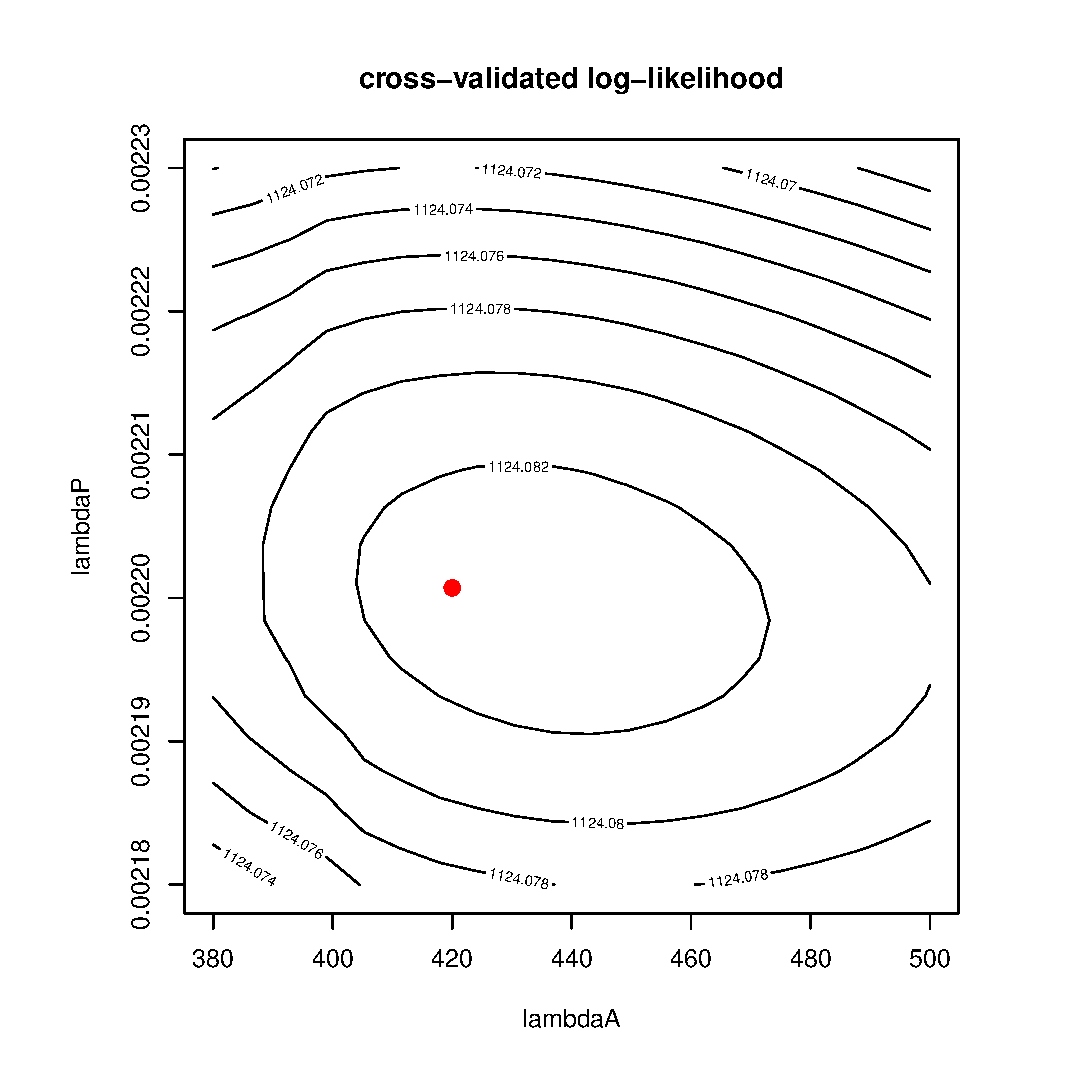
\includegraphics[scale=0.33]{contPlot.eps}&
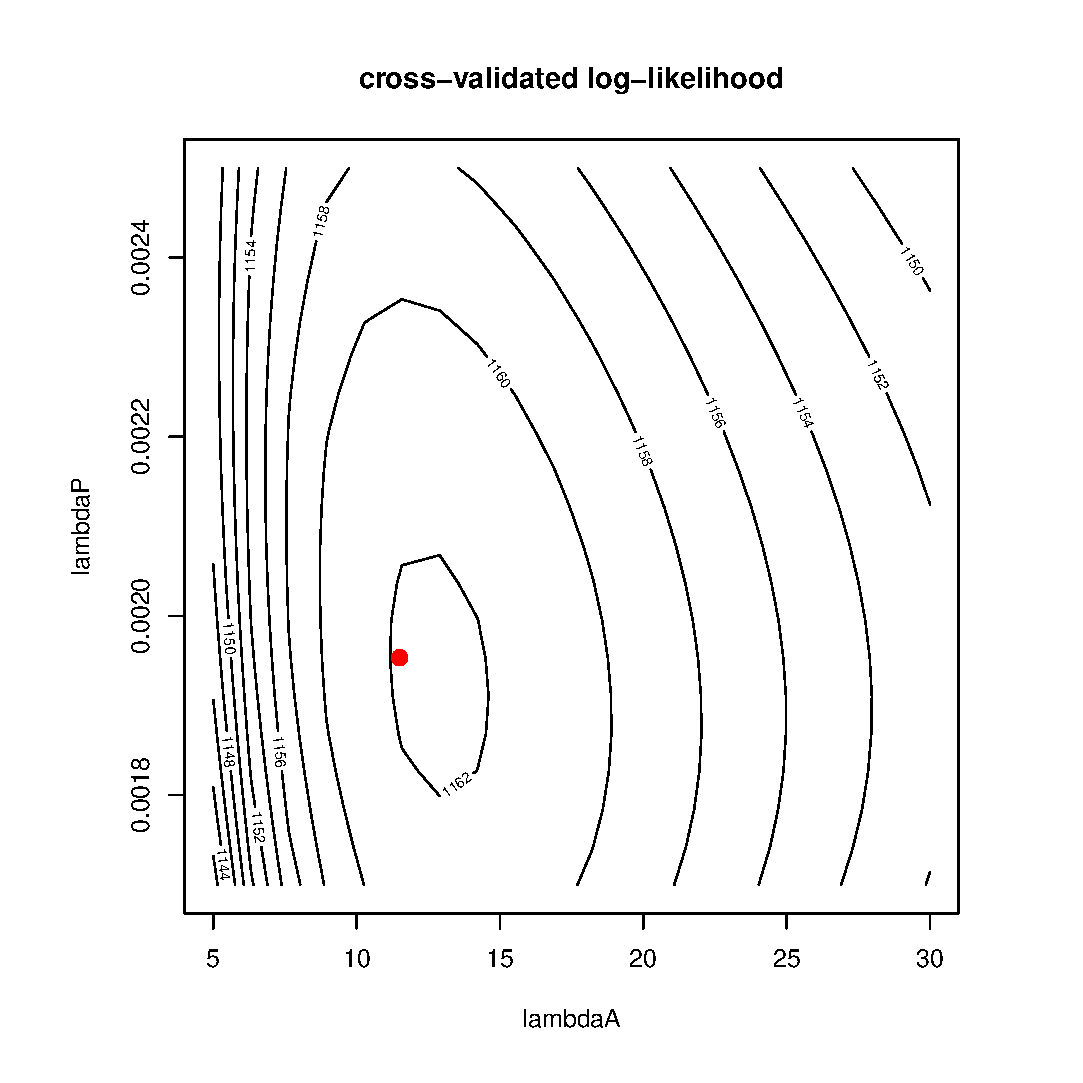
\includegraphics[scale=0.33]{contPlot_rf.eps}\\
\end{tabular}
\caption{Contour plots of LOOCV log-likelihood of VAR(1) model for p53 signaling pathway. Left panel represent the contour plot of the penalty parameter in the first estimation, while in the right panel the contour plot of the re-estimated parameters}
\label{fig:contour}
\end{figure}

Model parameters are estimated as outlined in the Section 3. First, optimal penalty parameters are determined through maximization of the LOOCV log-likelihood, resulting in $\lambda_a=420.0000$, $\lambda_{\omega}= 0.0022$. Figure \ref{fig:contour} shows the contour plot of the LOOCV log-likelihood of VAR(1) model. The red dot in Figure \ref{fig:contour} represents the penalty parameter choice. According the contour plot the red dot is close to the maximum, implying the employed optimization procedure has converged. With these optimal penalty parameters the ridge penalized maximum likelihood estimates of $\mathbf{A}$ and $\mathbf{\Omega}_{\varepsilon}$ are obtained. These estimates are illustrated as heatmaps in Figure \ref{fig:ridgeAP}. 

\begin{figure}[h!]
\centering
\begin{tabular}{cc}
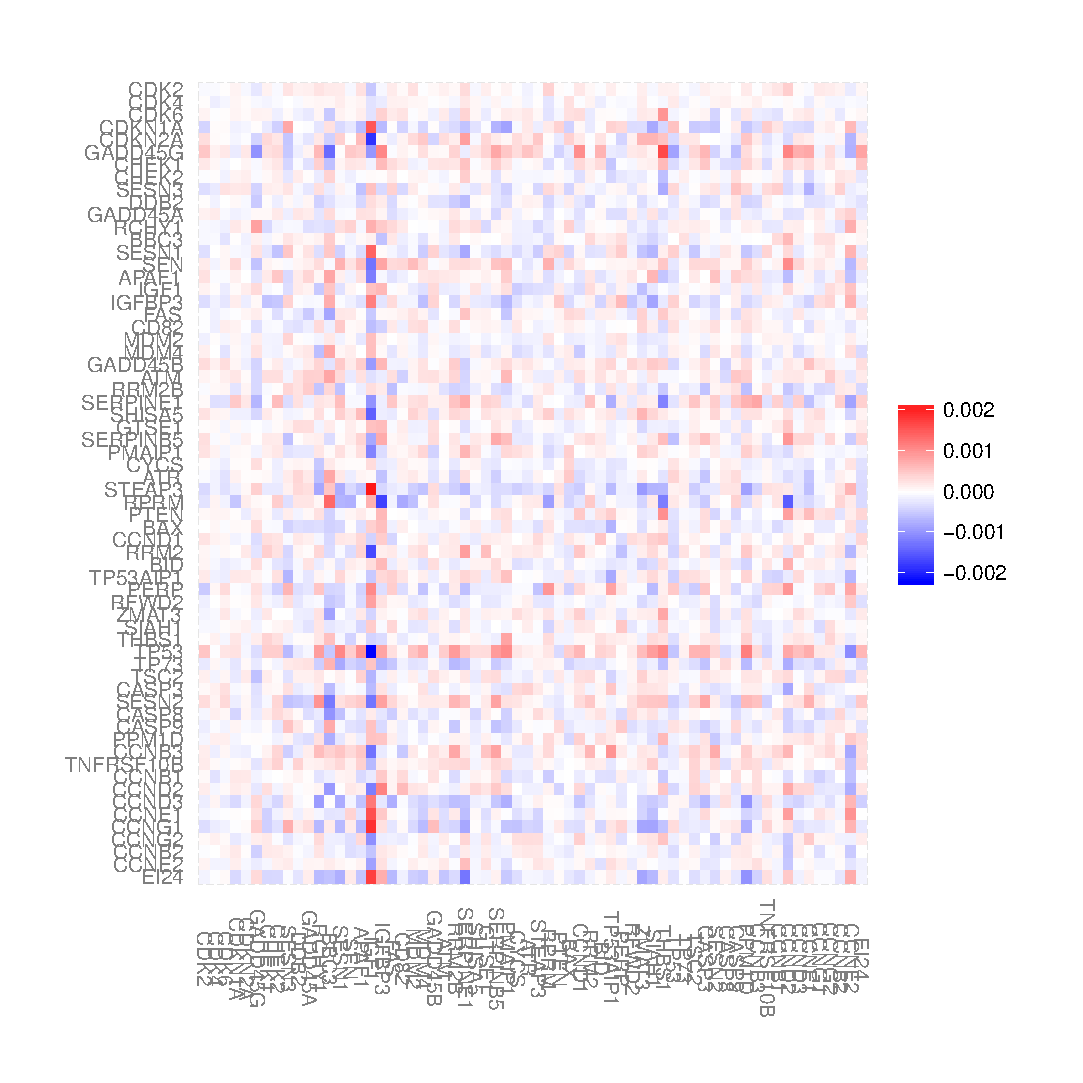
\includegraphics[scale=0.33]{ridgeA.eps}&
\includegraphics[scale=0.33]{ridgeP.eps}\\
\end{tabular}
\caption{ Heat maps of the estimated parameters for p53 signaling pathway using proposed method. Left panel represent estimates for $\mathbf{A}$, while right panel for $\boldsymbol{\Omega_{\varepsilon}}$. Each element of the heatmap represents, an edge, with intensity of positive or negative effect between two genes. In biological contexts positive(negative) effect mean that one gene activate(repress) another gene.
}
\label{fig:ridgeAP}
\end{figure}

To facilitate biological insight genes with the strongest temporal and contemporaneous relations are singled out through post-estimation support determination of $\mathbf{A}$ and $\mathbf{\Omega}_{\varepsilon}$ (confer Section 4.2). For the selection of nonzero elements, corresponding to edges in the time series chain graph, of $\mathbf{A}$ and $\mathbf{\Omega}_{\varepsilon}$ a cut-off of $1-\widehat{\textrm{lFDR}}\geq 0.999$ is applied. This high cut-off results in a sparse and interpretable graph. Figure \ref{fig:ridgeAPspar} displays the selected edges as a heatmap. Red squares in the heatmap represent (significant) edges between two genes. The heatmap reveals the presence of genes with either a horizontal or vertical red stripy pattern. Genes (e.g. CGKN2A, TP53,TP73, CGKN1A, GADD45G) with the horizontal stripes can be thought of as the `regulatees' in the pathway, while the vertical ones (e.g. IGF1, IGFBP3, BBC3, CCND2, THBS1) are the `regulators' of the pathway. This is confirmed when studying node statistics (like in- and out-degree, betweenness, centrality, confer Newman for definition (\cite{Newman2010})) derived from the inferred graph (Table \ref{table:postEst}).

\begin{figure}[h!]
\centering
\begin{tabular}{cc}
\includegraphics[scale=0.33]{ridgeAspar0999.eps}&
\includegraphics[scale=0.33]{ridgePspar0999.eps}\\
\end{tabular}
\caption{Heat maps of sparsified parameter estimates for p53 signaling pathway using proposed method. Left panel represent estimates for $\mathbf{A}$, while right panel for $\boldsymbol{\Omega_{\varepsilon}}$.}
\label{fig:ridgeAPspar}
\end{figure}

With knowledge of their support less biased estimates of $\mathbf{A}$ and $\mathbf{\Omega}_{\varepsilon}$ are obtained by a refitting them taking the support into account. Optimal penalty parameters are re-determined: $\lambda_a=11.4000$, $\lambda_{\omega}= 0.0019$ (and confirmed by the contour plot the LOOCV log-likelihood, Figure \ref{fig:contour}). The re-estimated parameter $\mathbf{A}$ is visualized as a heatmap (Figure \ref{fig:ridgeArf}). The temporal relations among the genes are also visualized in form of a graph (confer  Figure  \ref{fig:graph}), where edges represent the effect of the expression levels of a gene at timepoint $t$ to that of another genes at time point $t+1$.  

\begin{figure}[h!]
\centering
\begin{tabular}{cc}
\includegraphics[scale=0.33]{ridgeArf.eps}&
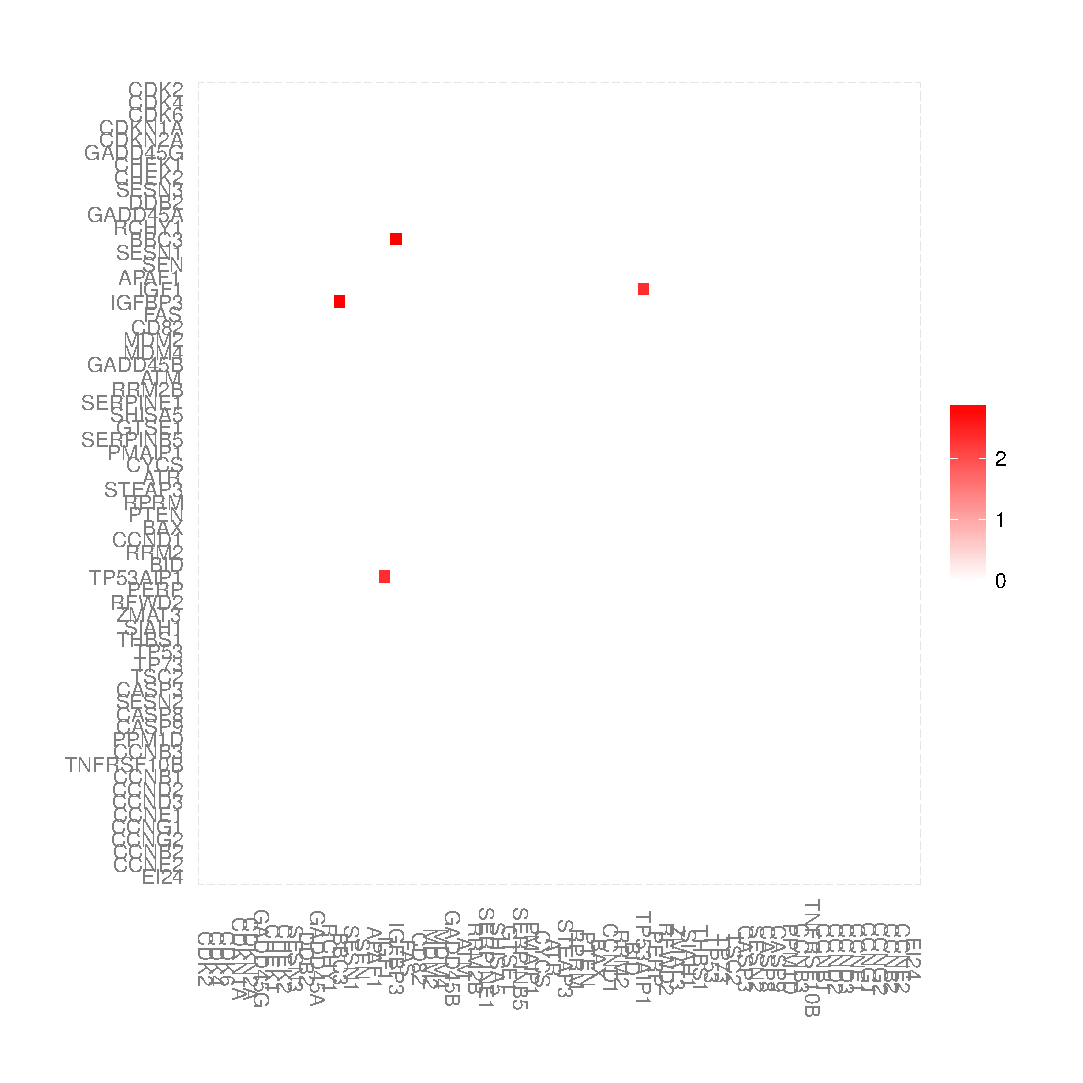
\includegraphics[scale=0.33]{ridgePrf.eps}\\
\end{tabular}
\caption{Heat maps of re-fitted parameter estimates for p53 signaling pathway using proposed method incorporating the prior knowledge on the support on $\mathbf{A}$.}
\label{fig:ridgeArf}
\end{figure}

\begin{figure}[h!]
\centering
\begin{tabular}{c}
\includegraphics[scale=0.4]{graph.pdf}\\
\end{tabular}
\caption{Graphs of the temporal relations among the genes as implied by the parameter estimates of $\mathbf{A}$ for p53 signaling pathway.
Solid line represent positive effect, while dashed lines negative effect. Thickness of the lines indicate how strong is the effect. For the sake of the graph clarity, genes which are not connected with edge to another genes are omitted.
}
\label{fig:graph}
\end{figure}

Employing the re-estimated parameter $\mathbf{A}$, we study the fit ($\hat{\mathbf{Y}}_{\ast, i, t} = \hat{\mathbf{A}} \mathbf{Y}_{\ast, i, t-1}$) of the `regulatees' (genes explained by other genes). Figure \ref{fig:fitTP73} shows the expression levels of the up-regulated gene TP73 along with its fit (red line) in the four cell lines (one panel each). Considering the use of a linear model, the fit captures the salient features of the data. The fit is studied for all genes in the pathway. The result is summarized in Figure \ref{fig:corFitObs}. It displays the histogram of the Spearman correlations between the fit and the observations, cell line-wise. The histogram in Figure \ref{fig:corFitObs} is clearly skewed to the domain $[0,1]$. This indicates that the fit is generally reasonable.

\begin{figure}[h!]
\centering
\begin{tabular}{cc}
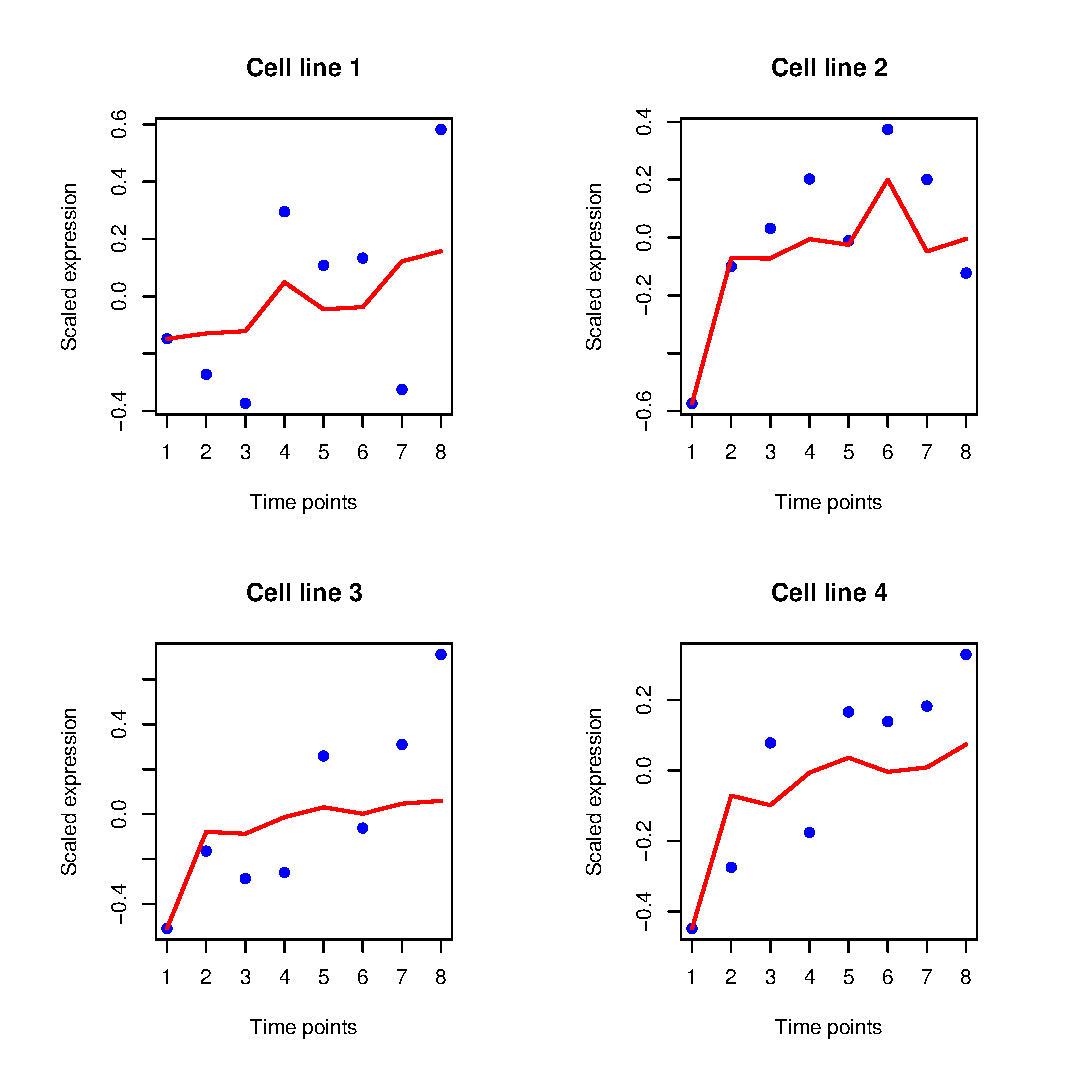
\includegraphics[scale=0.7]{fitTP73.eps}\\
\end{tabular}
\caption{Fit of the expression levels of TP73 over time in all cell lines. Dots represent the expression levels, while solid red lines indicated the fit of the model over time.}
\label{fig:fitTP73}
\end{figure}

\begin{figure}[h!]
\centering
\begin{tabular}{cc}
\includegraphics[scale=0.5]{corFitObs.eps}\\
\end{tabular}
\caption{Histogram of the correlation between model fit and observation of data set from the p53 signaling pathway.}
\label{fig:corFitObs}
\end{figure}


With final and less-biased estimates of the VAR(1) parameters at hand, we study the quantitative, dynamic implications of the model: what are the down-stream effects of a change in expression levels of a gene? This can be done through impulse response analysis (confer Section 4.2 for details). For each gene the column-wise average of the (absolute) impulse response on all other genes at the next time instance is calculated (Table \ref{table:postEst}). This is a measure of a gene's driving force on the pathway's expression levels. The low and high impulse responses of the $\{$ CGKN2A, TP53,TP73, CGKN1A, GADD45G $\}$ and $\{$ IGF1, IGFBP3, BBC3, CCND2, THBS1 $\}$ genes corroborate with their interpretations of `regulatees' and `regulators'. This is supported when evaluating the mutual information between each gene at time point $t$ and the whole pathway at next time point (Table \ref{table:postEst}). 

\begin{table}
\caption{Gene statistics for the top genes(in terms of the number of edges) for p53 signaling pathway; in-degree of A - number of (temporal) edges pointing to each gene; out-degree of A - number of (temporal) edges leaving each gene; centrality - eigenvector centralities of the gene within the graph;
impulse response - absolute impulse response in the first time point;
mutual information - mutual information in the first time point
}
\begin{tabular}{l*{6}{c}r}
\hline
\hline          
             &\textbf{in-deg.} &\textbf{out-deg.} & \textbf{cent.} & \textbf{imp. resp.} & \textbf{mut. inf.}  \\
\hline
IGF1        & 0 & 25 & 1.0000 & 0.01245 &0.0124\\
IGFBP3      & 0 & 11 & 0.7555 & 0.0039 & 0.0027\\
BBC3       & 0 & 9 & 0.4502 & 0.0037 & 0.0034 \\
CCND2    & 0 & 7 & 0.5353 & 0.0015 & 0.0010 \\
THBS1    & 0 &7 & 0.7892  &0.0030 & 0.0044 \\
CDKN2A    & 8 & 0 & 0.3993 & 0 & 0  \\
TP53    & 7 & 0 &0.2595 & 0 & 0\\
TP73   & 5 & 0 & 0.2595 & 0 & 0\\
CDKN1A       & 5 & 0 & 0.2714 & 0 & 0\\
GADD45G      & 5 & 0 & 0.2820  & 0 & 0\\
\hline
\end{tabular}
\label{table:postEst}
\end{table}

The downstream effects of a signal may be further elucidated through the decomposition of the covariance between the expression levels of two genes in terms of the paths connecting them in the time-series chain graph (as described in Section 4.3). For illustration purposes consider the regulator-regulatee pair (IGFBP3, TP73) at two contiguous time points. They are connect through two paths: a direct path $(Y_{\mbox{{\tiny IGFBP3}},t} \rightarrow Y_{\mbox{{\tiny TP73}},t+1})$ and an indirect one through $Y_{\mbox{{\tiny IGFBP3}},t} \rightarrow Y_{\mbox{{\tiny BBC3}},t}\rightarrow Y_{\mbox{{\tiny TP73}},t+1}$ (depicted in Figure \ref{fig:motifs}). The covariance the (IGFBP3, TP73) gene pair at contiguous time point may now decomposed as:
\begin{eqnarray*}
\mbox{Cov}(Y_{\mbox{{\tiny IGFBP3},t}},Y_{\mbox{{\tiny TP73},t+1}}) & = & (\boldsymbol{\Sigma}_{\varepsilon} \textbf{A}^\top)_{\mbox{{\tiny IGFBP3}}, \mbox{{\tiny BBC3}}} 
\\
& = & -0.003168001 \, \, \, = \, \, \, -0.002483485  - 0.0006845158, 
\end{eqnarray*} 
in which the two summands on the right-hand side correspond the direct and indirect path in the time-series chain graph. Based on the paths' contribution the direct one dominates, but being of the same sign the indirect path also contributes in the suppression of the expression levels of the TP73 gene.


Another way to grasp the inferred networks of the p53 signaling pathway is to study its motifs. Motifs are small recurring network patterns and form the building blocks of pathways (\cite{Alon2007}). As the inferred network is very sparse only few (three gene) motifs are found (Figure \ref{fig:motifs}). All these motifs are so-called feedforward loops (FFL), which appear in many gene systems (\cite{Alon2007}). Identified FFL motifs are all of the incoherent type, which connect two genes via two paths that have opposite effects:  positive (activating) and negative (repressing). A FFL motif found in the reconstructed time-series chain graph of the p53 signaling pathway is shown in Figure 
\ref{fig:motifs}. Here, gene IGF1 activates both SESN1 and TP73, while SESN1 represses TP73 gene. IGF1 and SESN1 thus affect TP73 in opposite ways. In the extreme case, when the effect of the SESN1 is equal to that of IGF1, this results (with a slight delay due to the time) in the repression of the TP73, reducing its expression levels to (virtually) zero (confer \cite{Alon2007}). To contrast this, a coherent FFL (e.g. SESN1 affect TP73 in a positive manner) with increased effects in the IGF1 and SESN1 gene, propagate delayed amplification of the signal in the TP73 (for more details see SM).

% \textcolor{blue}{SM:
% In order to gain more understanding on the effect of the FFL on the three gene pathway we performed small simulation study. Data from incoherent and coherent FFL are simulated at 100 time points for genes X, Y and Z. In the incoherent FFL, gene X have positive effect on the genes Y and Z, while Y negatively effect Z. Data for X are simulated from sin function, while $Y_{t} =X_{t-1}+\varepsilon_{t}$ and $Z_t=X_{t-1}-Y_{t-1}+\varepsilon_{t}$. Left panel in the Figure \ref{fig:FFLs} illustrate simulated data from incoherent FFL. From the figure we can notice that, due to the same level of the increased opposite effects of the X and Y, generate in the decreased signal in Z. On the other hand, in the coherent FFL gene X have positive effect on the genes Y and Z, while Y positively effect Z. Similarly, signal in X is represented as sin function, where $Y_{t} =X_{t-1}+\varepsilon_{t}$ and $Z=X_{t-1}+Y_{t-1}+\varepsilon_{t}$. Right panel in the Figure show simulated data from the coherent FFL. Due to the increased positive effect of X and Y on Z, signal in Z amplified.} 

% \begin{figure}[h!]
% \centering
% \begin{tabular}{cc}
% \includegraphics[scale=0.3]{incohFFL.eps}&
% \includegraphics[scale=0.3]{cohFFL.eps}\\
% \end{tabular}
% \caption{Simulated data of three genes from incoherent and coherent FFL are % plotted against 100 time points. }
% \label{fig:FFLs}
% \end{figure}


\begin{figure}[h!]
\centering
\begin{tabular}{cc}
%\includegraphics[scale=0.18]{Motif1.pdf}&
\includegraphics[scale=0.3]{Motif2.pdf}\\
%\includegraphics[scale=0.18]{Motif3.pdf}&
%\includegraphics[scale=0.18]{Motif4.pdf}\\
%\includegraphics[scale=0.18]{Motif5.pdf}&
%\includegraphics[scale=0.18]{Motif6.pdf}\\
\end{tabular}
\caption{Motifs of p53 signaling pathways.}
\label{fig:motifs}
\end{figure}








\newpage
\bibliographystyle{plainnat} % Style BST file

\bibliography{bio_article} % Bibliography file (usually '*.bib' )

\end{document}

